\chapter{Local Guide}

\emph{This guide was written by Kevin Cohen. For the most up-to-date
  version, please visit
  \url{http://bretonnel.com/2015/04/29/visiting-denver-for-naacl2015/}.}
\index{Cohen, Kevin B.}

The North American Association for Computational Linguistics annual
meeting (NAACL 2015) will be held in Denver, Colorado this year. Here
are some things that I think might be useful or enjoyable for visiting
computational linguists, natural language processing people, and the
like. I'm not going to talk about the mountains, Red Rocks, or any of
that kind of stuff---you can find that in tourist guides, hotel
propaganda, and pretty much anywhere else.  These are some of the
things that make life in Denver bearable, and that I don't think
you'll hear about elsewhere.

\paragraph{Airport}

The Denver International Airport looks quite distinctive. Opinions
differ as to whether it is meant to look like teepees, the Rocky
Mountains, or what. It features in a number of conspiracy theories,
which mainly claim that it is built over an underground complex that
will be the seat of the government of the New World Order. On the way
from the airport to Denver, be sure to look for the Demon Horse
statue. We call it the Demon Horse for two reasons: (1) it has glowing
red eyes, and (2) during its construction, the head fell off and
crushed the artist, killing him.

\paragraph{Bookstores}

Here's a link to a web page listing ten good or great independent
Denver bookstores:

\url{www.westword.com/arts/the-ten-best-bookstores-in-denver-6659360}

\paragraph{Bars}

The classic Denver bar that no one else knows about is El Chapultepec.
Either arrive early, or be prepared to stand all evening. You can
reach it from the conference hotel with a ride down the 16th Street
Mall free shuttle and a short walk through a lively neighborhood. The
LoDo area has many bars that are quite busy on weekend nights. Use
caution around the time that the bars close. Again, you can reach
LoDo quite easily from the conference hotel via the free 16th Street
Mall shuttle.

\paragraph{Restaurants}

A rare hippie restaurant treat in Denver is the Mercury Cafe, known to us locally as “The Merc.”  It's a step back into the 1960s, sorta.  Take a cab there, or the light rail–don't try to walk from the conference hotel, as the neighborhood is not always safe.

\paragraph{Marijuana}

Marijuana is legal here under state law. You can find it easily; the
stores (usually known as “dispensaries”) are typically marked with a
green cross or a green marijuana leaf. However, it is NOT legal under
federal law---if you are not an American citizen, don't take a chance
with this. It's a legal gray zone, and people do occasionally get
burnt. Also, like alcohol, it is not legal to consume it in public.
(And, no: I don't indulge!)

\paragraph{Mexican food}

The Denver population is 30\% Hispanic, and we have fantastic Mexican
food here---also Salvadoran and some Peruvian, if you don't mind
leaving the area of the conference hotel to find it. Mexican food is
an integral part of American food in this part of the country. A good
place to get it is Real de Minas, on Colfax. Avoid the
cheese-smothered burrito platters and have something that's actually
Mexican, like tacos de carne asada, or ribs (costillas) in green chile
sauce. You can get there on the number 15 bus---more on that below.

\paragraph{Decadent snacks}

Voodoo Doughnuts is an import from Portland, Oregon–some of you may
remember it from ACL 2011. Truly amazing doughnuts---be prepared to
stand in line. You can get there on the number 15 bus from the
conference hotel.

\paragraph{Local beers}

Denver has a lot of microbreweries, and many good local beers. One of
the main favorites is Fat Tire (which is now nationally distributed,
so you may have had it before).

\paragraph{The Number 15 bus}

The number 15 bus goes up and down Colfax Avenue, allegedly the
longest street in America, and probably one of the sleaziest. (Colfax
runs quite close to the conference hotel.) Everyone in Denver has a
story about the number 15 bus, typically involving a drunk, a drug
addict, or vomit. It's actually pretty safe, although you should be
careful on Colfax at night, as you would in any big city anywhere in
the world. The last stop on the eastbound leg of the route (away from
the mountains) is the Anschutz/Fitzsimons medical campus. Stop by the
Biomedical Text Mining Group in the Center for Computational
Bioscience for one of the best views of downtown Denver and the
mountains that you'll find.

\paragraph{Safety}

Denver is a pretty safe city. Aurora is not quite as safe,
particularly in the older parts of town. In general, you should be
aware of your surroundings in the evening, as you would be in any big
city.

\pagestyle{empty}
\begin{center}
  \clearpage
  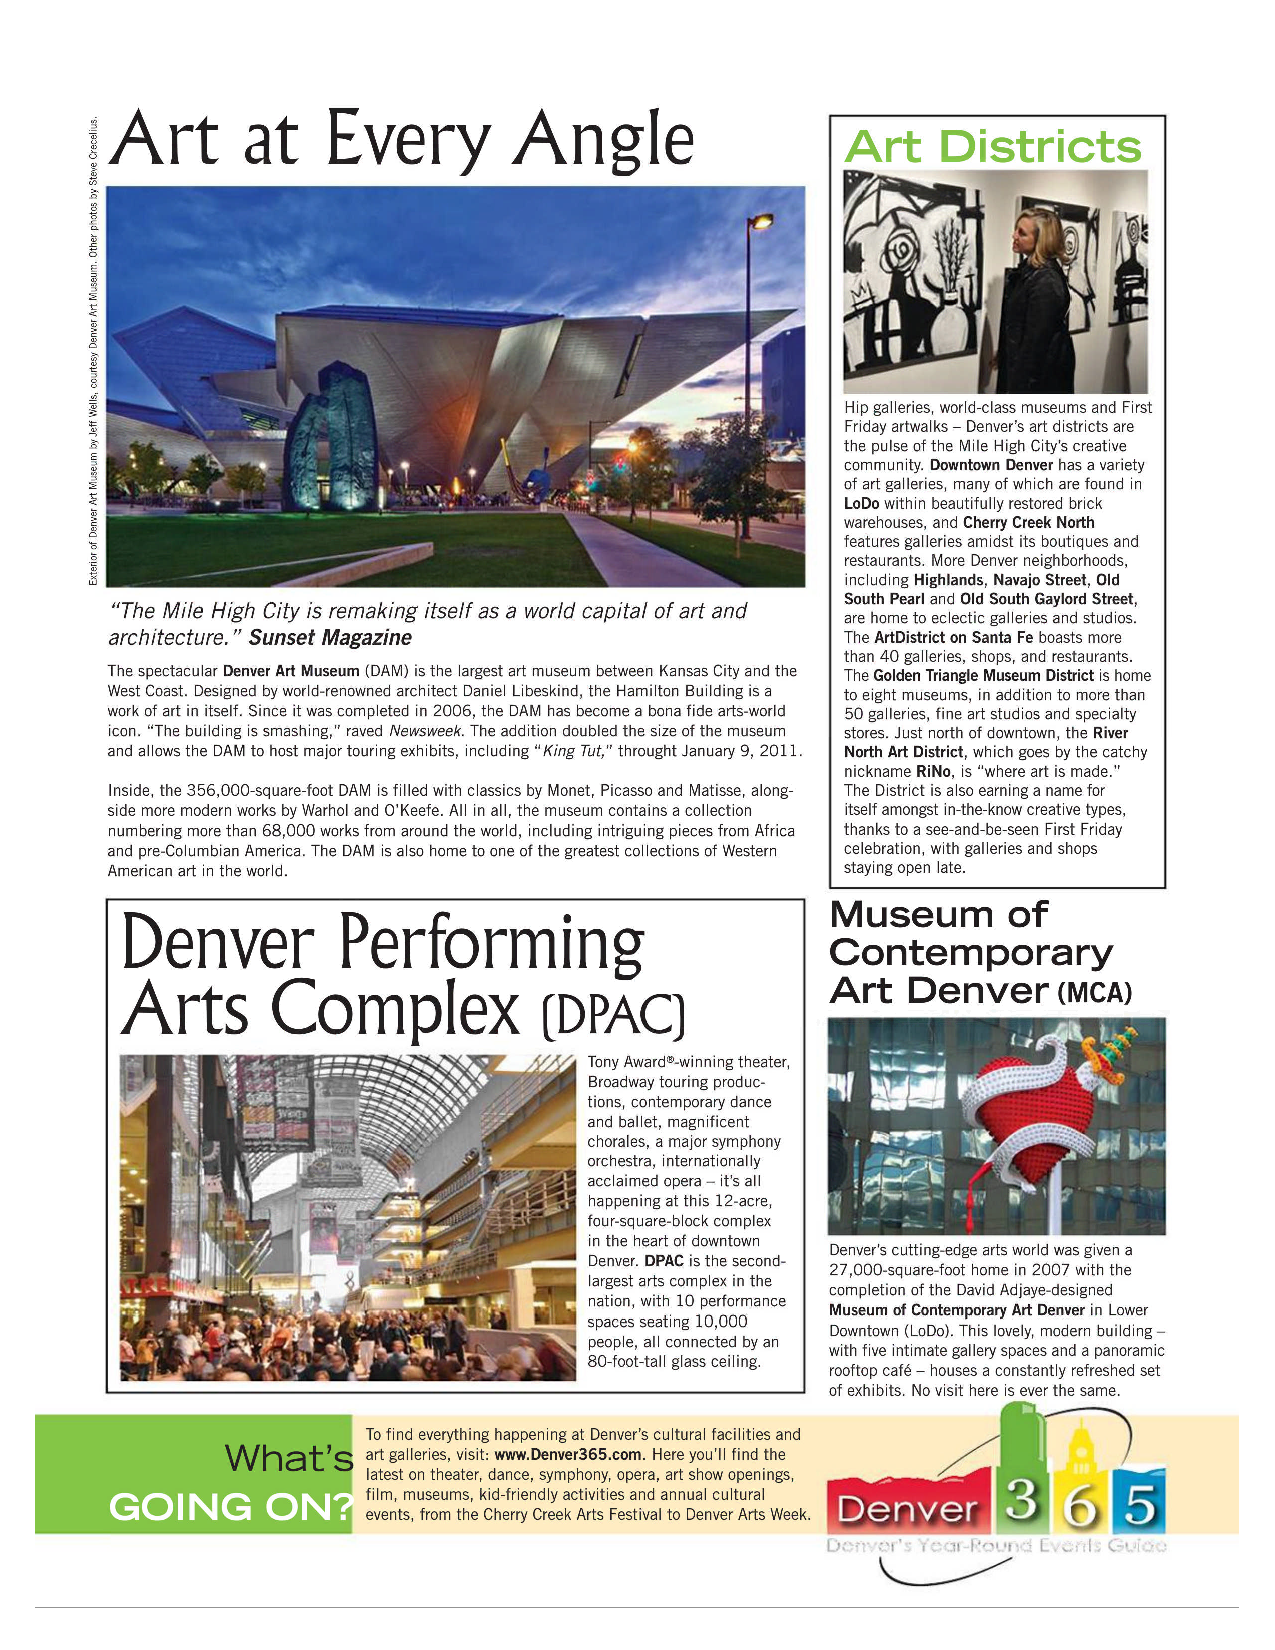
\includepdf[pages={1},width=5in]{content/local-guide/Arts.pdf}
  \clearpage
  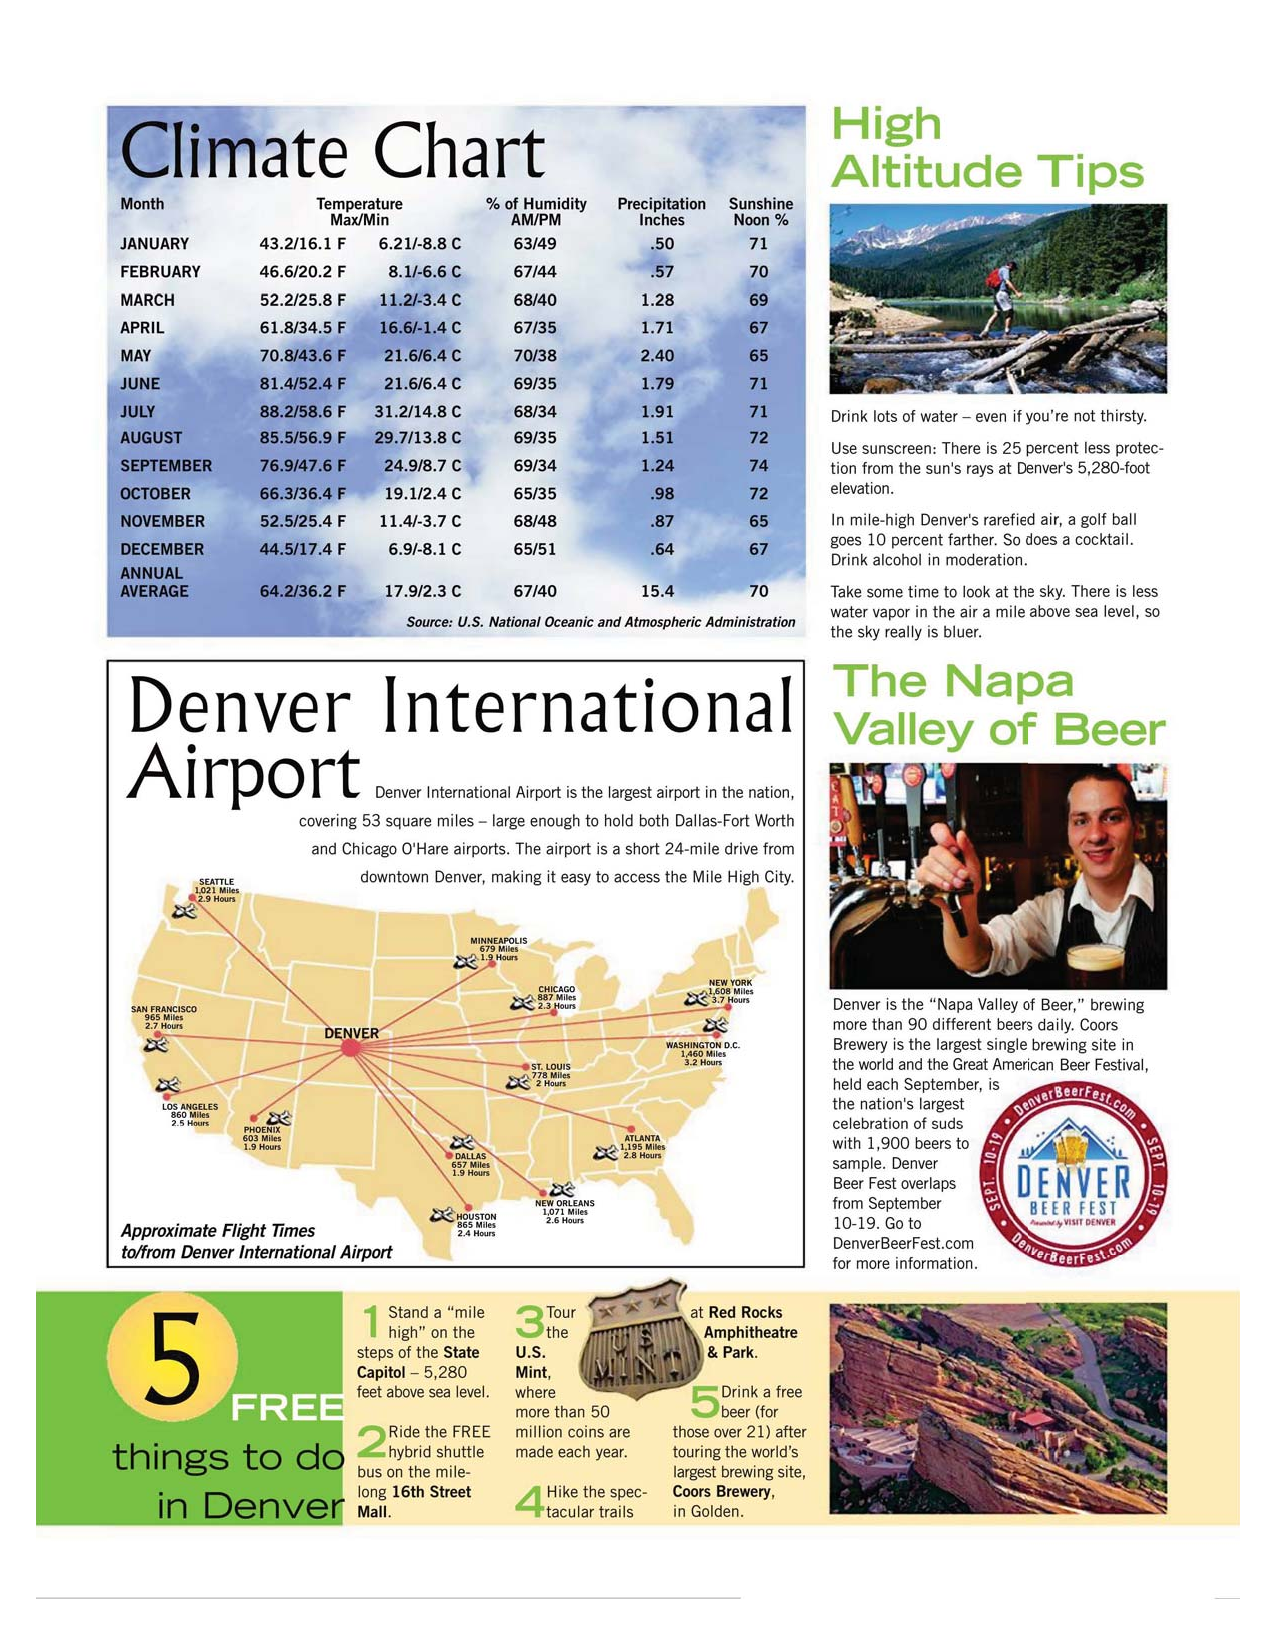
\includepdf[pages={1},width=5in]{content/local-guide/Climate.pdf}
  \clearpage
  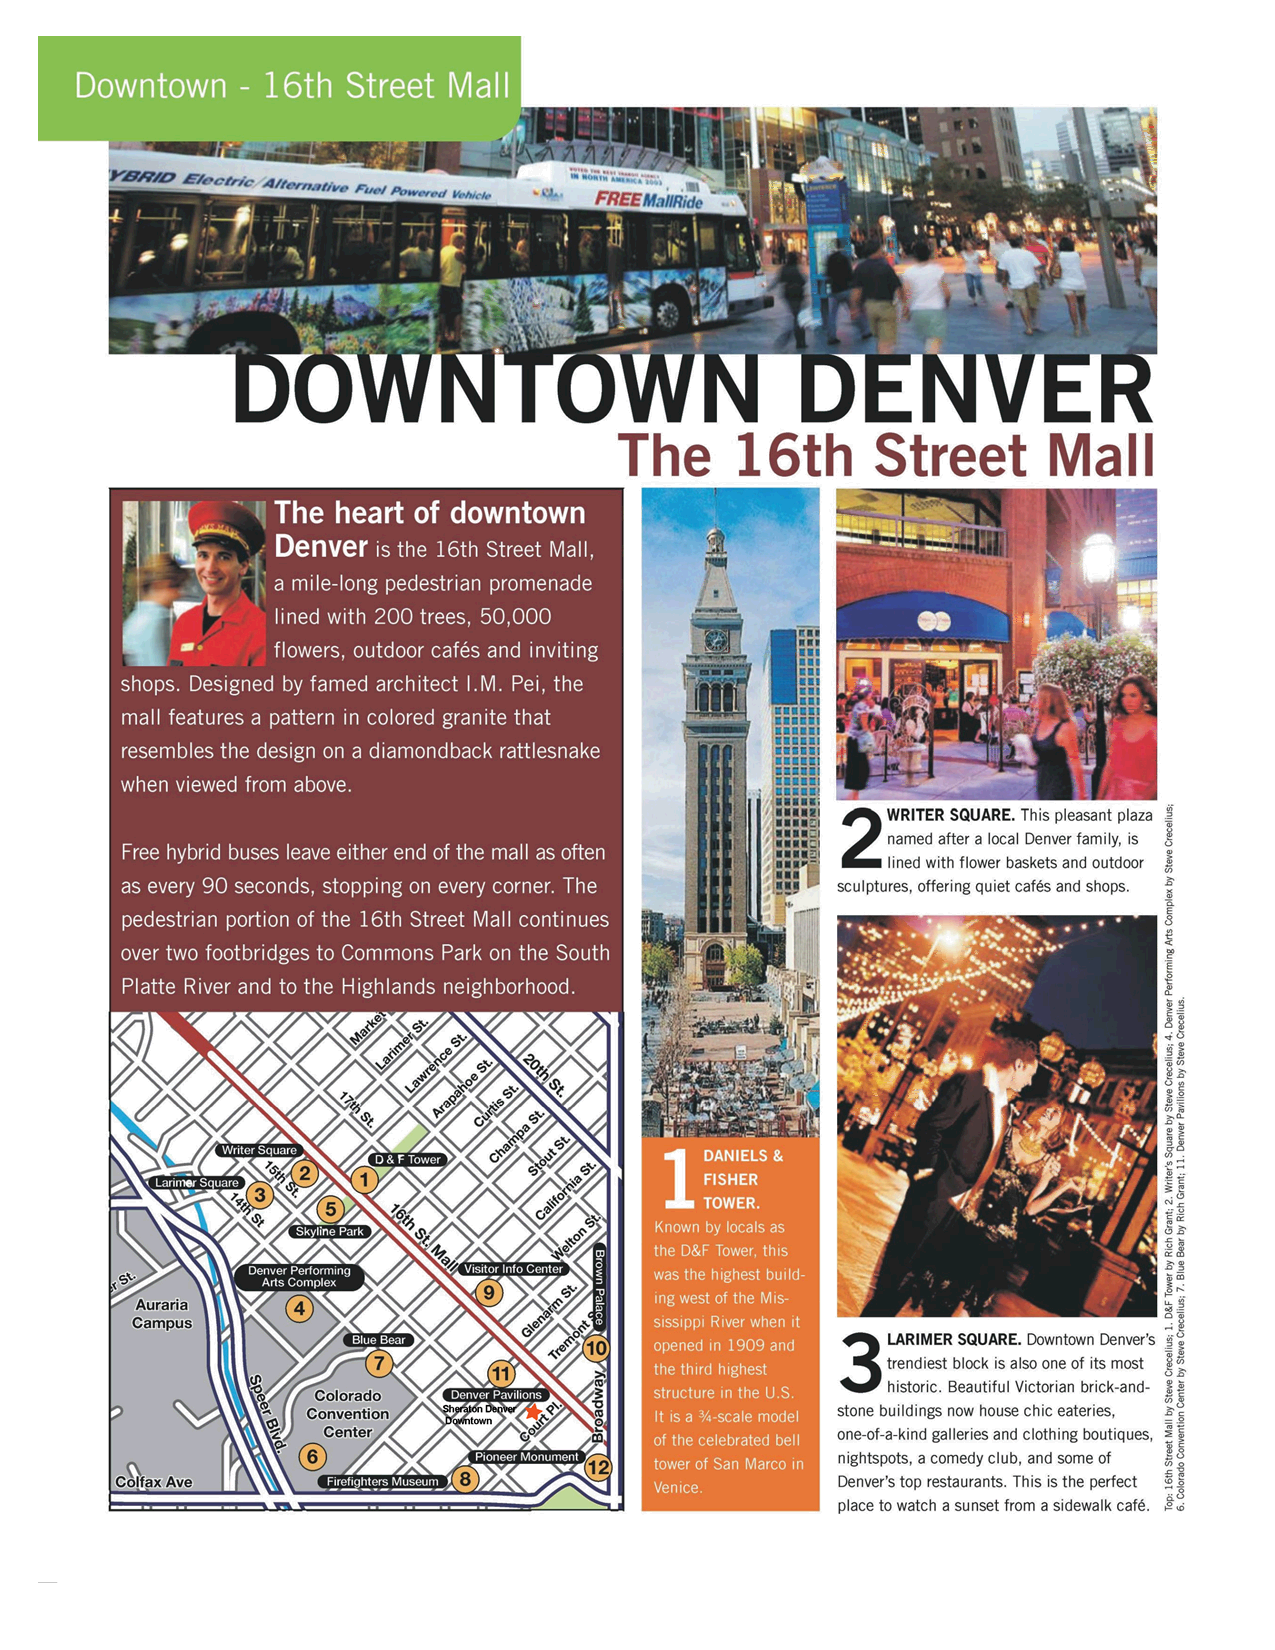
\includepdf[pages={1},width=5in]{content/local-guide/mall-1.pdf}
  \clearpage
  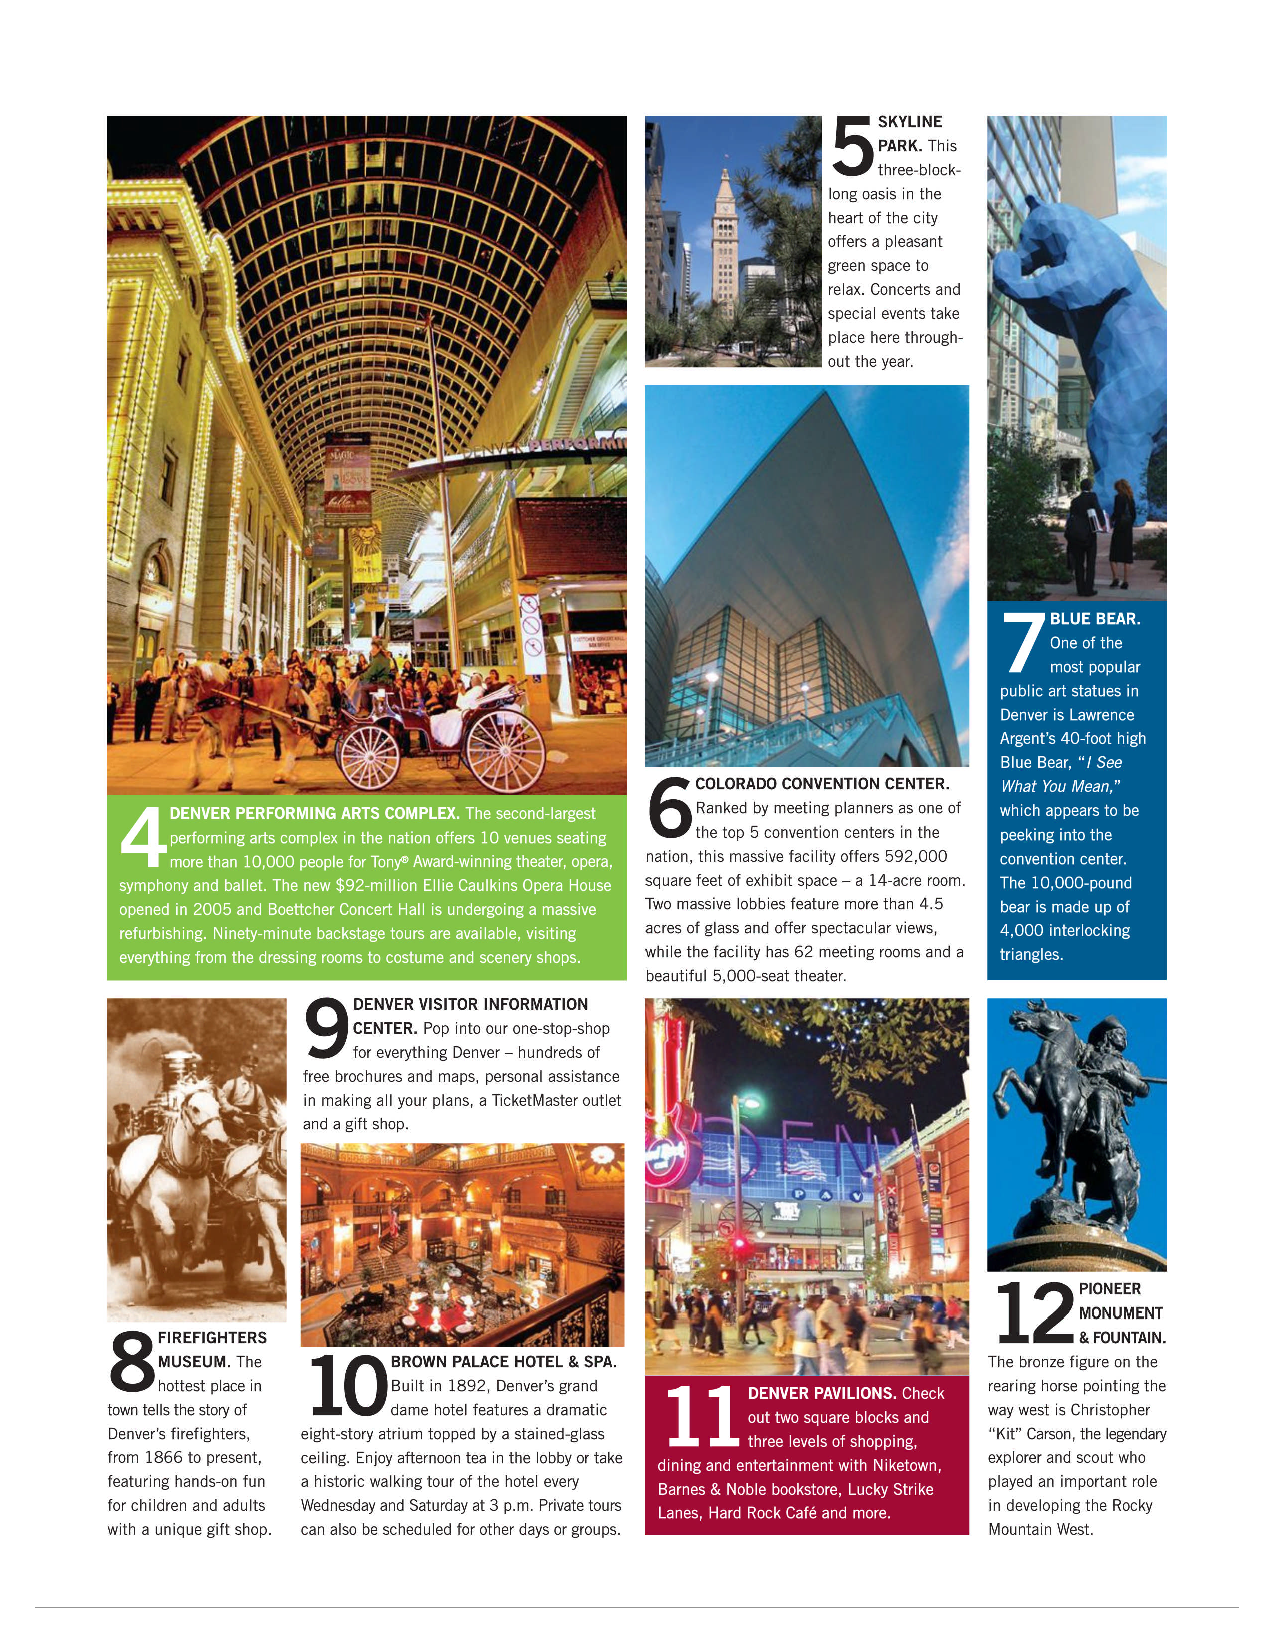
\includepdf[pages={1},width=5in]{content/local-guide/mall-2.pdf}
  \clearpage
  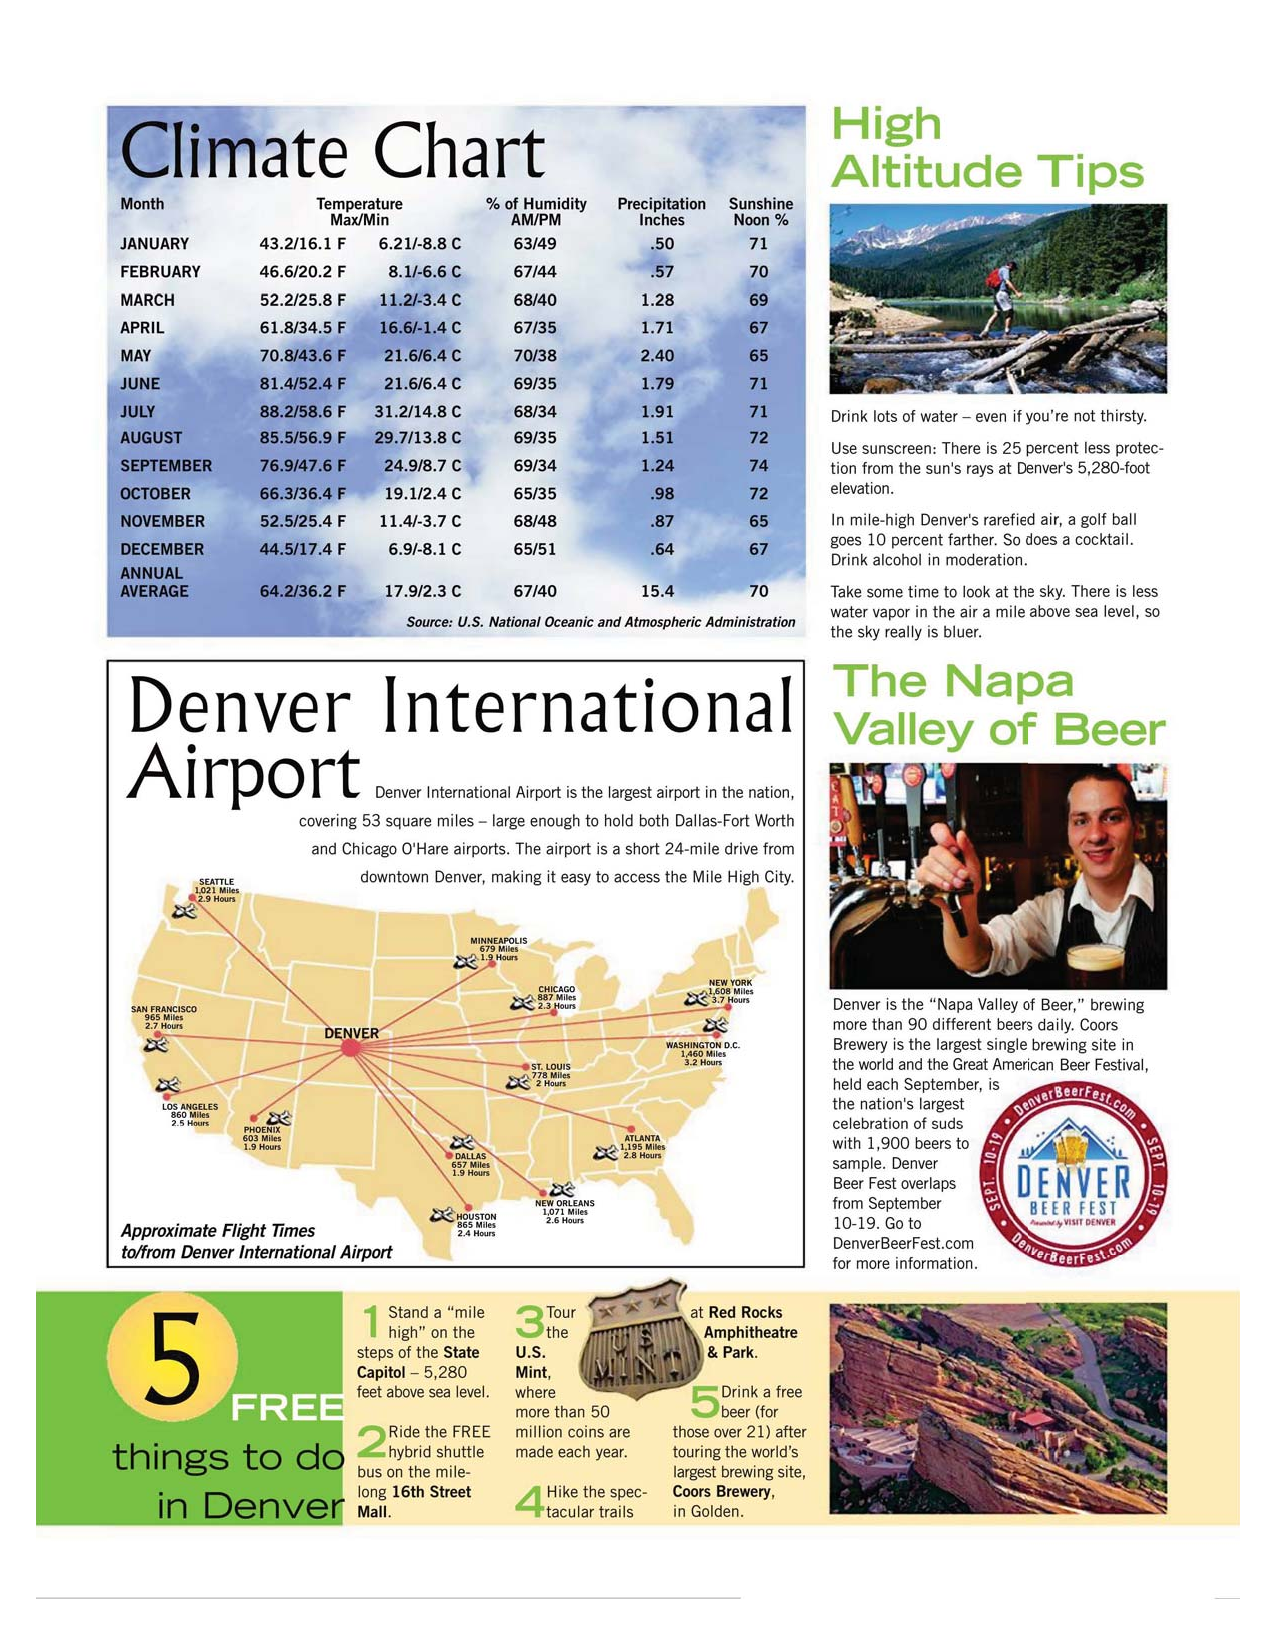
\includepdf[pages={1},width=5in]{content/local-guide/Climate.pdf}
  \clearpage
  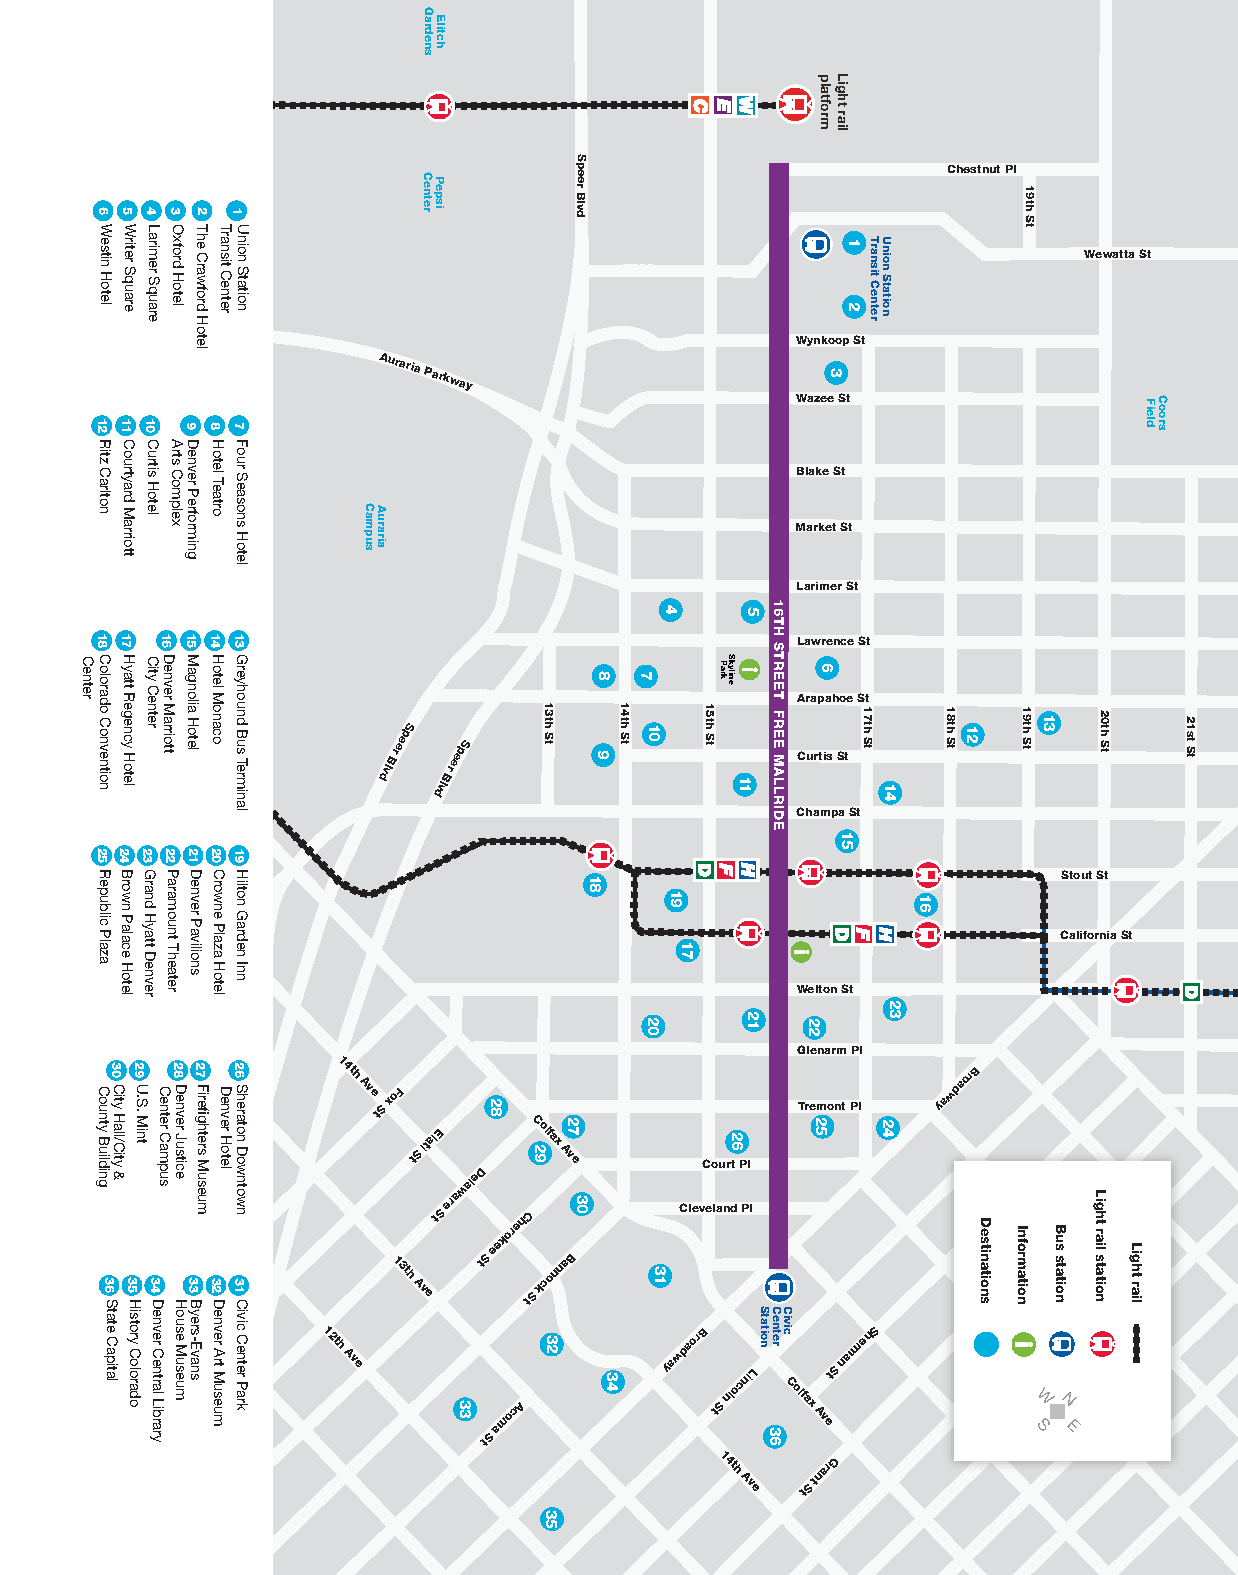
\includepdf[pages={1},width=5in]{content/local-guide/FreeMallRideMap.pdf}
\end{center}
